\documentclass[border=2mm]{standalone}
\usepackage{tikz}
\begin{document}
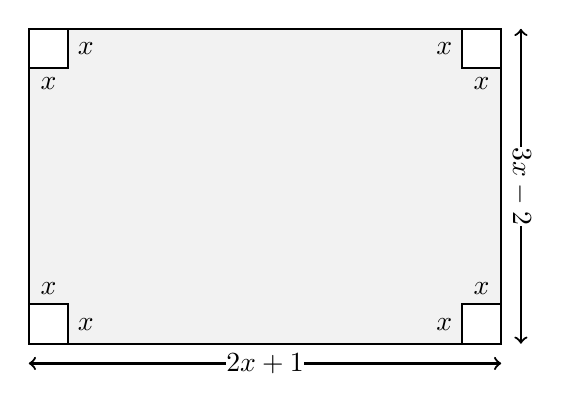
\begin{tikzpicture}
   %\draw[step=1cm,gray,very thin] (-1,-1) grid (7,5);
   
   \filldraw[gray!10!white, thick, draw=black] (0,0) rectangle (6,4);
   \node at (3,-0.25) {$2x+1$};
   \node [ rotate=270] at (6.25,2) {$3x-2$};
   \draw [<-, thick] (0,-0.25) -- (2.5,-0.25);
   \draw [->, thick] (3.5,-0.25) -- (6,-0.25);
   \draw [<-, thick] (6.25,0) -- (6.25,1.5);
   \draw [->, thick] (6.25,2.5) -- (6.25,4);

   \filldraw[white, thick, draw=black] (0,0) rectangle (.5,.5);
   \filldraw[white, thick, draw=black] (0,3.5) rectangle (0.5,4);
   \filldraw[white, thick, draw=black] (5.5,0) rectangle (6,0.5);
   \filldraw[white, thick, draw=black] (5.5,3.5) rectangle (6,4);
   
   \node [right] at (0.5,0.25) {$x$};
   \node [above] at (0.25,0.5) {$x$};
   
   \node [left] at (5.5,0.25) {$x$};
   \node [above] at (5.75,0.5) {$x$};

   \node [right] at (0.5,3.75) {$x$};
   \node [below] at (0.25,3.5) {$x$};

   \node [left] at (5.5,3.75) {$x$};
   \node [below] at (5.75,3.5) {$x$};

\end{tikzpicture}
\end{document}